\section{Analysis}
\label{sec:analysis}

We analyze performance of SMON in this section.

SMON uses epidemic algorithm to maintain itself. Peers will
initiate periodic communication to other random peers. We
will show that these maintenance tasks have good
performance and scalability. In the analysis, we assume that
SMON works in synchronized way, that is each peer performs
its maintenance tasks in synchronized rounds and the tasks
finish almost instantaneously. Although the real SMON system
works asynchronously, the analysis can still give insights
on performance of SMON design. We will also evaluate SMON in
real conditions (see section~\ref{sec:eval}) and validate
our analysis.

% performance and scalability

The epidemic algorithm has three variants, called push, pull
and push-pull, and they are used by different maintenance
tasks of SMON as summarized in table~\ref{tbl:tasks}.
Although they differ in details, the basic result of
epidemic theory shows that each one of the three methods can
eventually infect the entire population.  The studies also
show that starting from a single peer, this is achieved in
expected time (the rounds number) proportional to the log of
the population size ($\log N$).

\begin{table}
\centering
\begin{tabular}{|l|l|}

\hline
Self-deployment & push \\

\hline
Self-upgrade & push-pull \\

\hline
Self-recovery & push \\

\hline
Enable SMON & push \\

\hline
Disable SMON & pull \\

\hline
Application deployment & push-pull \\

\hline
\end{tabular}
\caption{Different variants of epidemic algorithm used by
maintenance task of SMON.}
\label{tbl:tasks}
\end{table}

Take self-deployment process as an example. Starting from a
single SMON peer, all the target machines will be deployed
with a SMON peer.  According to existing
studies~\cite{Eugster2004}, the self-deployment process can
be modeled as a branching process with population $n$. After
$r$ rounds, the expected fraction of deployed machines is:

\begin{equation*}
Y_r \approx \frac{1}{1+ne^{-r}}
\end{equation*}

The relation of $Y_r$ and $r$ is demonstrated in
figure~\ref{fig:yr}.

\begin{figure}
\centering
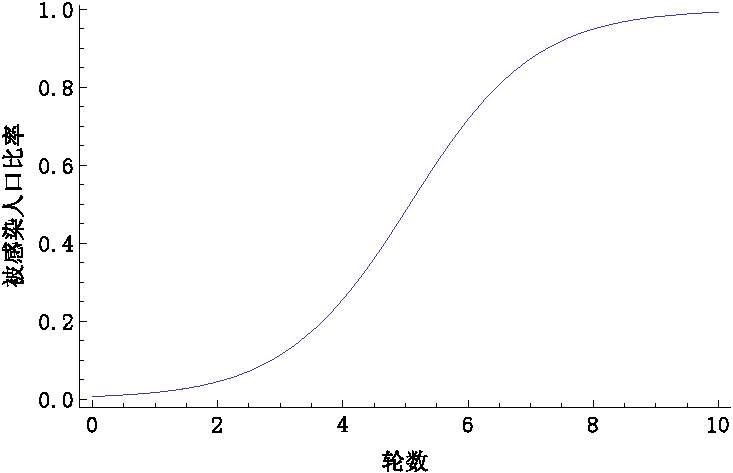
\includegraphics[scale=0.618]{Y_r}
\caption{Relation of expected infected population $Y_r$ with
round number $r$.}
\label{fig:yr}
\end{figure}


The ratio of deployed machines to un-deployed ones increases
exponentially, on average, by a factor of $e$ in each round.
This indicates that the self-deployment has good
performance.

To deploy a fix fraction of machines, the expected round
number $r$ is:

\begin{equation*}
r \approx \ln(n) - \ln(\frac{1}{Y_r} - 1)
\end{equation*}

$r$ is in the logarithm of total population $n$, which
implies good scalability of self-deployment process.

% overhead number

Another performance metric in concern is the overhead in
the self-deployment process. Since we use epidemic
algorithm, there may be duplicated deployed SMON peers in a
machine. Although there will be only one instance running,
the duplicated deployment will waste network resource and
disk storage at some extent.

We next show that the overhead is small on average (constant
actually). Assuming that there are $n$ machines in total,
and $m$ machines have been deployed already. For any one of
$n-m$ un-deployed machines, it may be selected by $k, (k <=
m)$ peers as the deployment target in the next round.  The
distribution of $k$ is can be expressed as binomial
distribition with parameter $(m, \frac{1}{n})$.

\begin{equation*}
P(X=k) = C_m^k (\frac{1}{n})^k (1 - \frac{1}{n})^{m - k}
\end{equation*}

We define the simultaneous deployment number $k, (k > 0)$ as
the deployment overhead. It is the conditional probability
when $k > 0$.

\begin{equation*}
\begin{aligned}
P(X' = k) &= P(X=k | X > 0) \\
&= P(X = k) / (1 - P(X = 0)) \\
&= P(X = k) / (1 - (1 - \frac{1}{n})^{m}) \qquad (k > 0)
\end{aligned}
\end{equation*}

The expectation of $k$, the overhead number, is:

\begin{equation*}
\begin{aligned}
E(X') &= \sum_{k=1}^m k \cdot P(X=k|X>0)  \\
      &= \frac{1}{(1 - (1 - \frac{1}{n})^{m})} E(X)
\end{aligned}
\end{equation*}

Further, note that when $n$ is large, and $m$ is approaching
$n$, we have

\begin{equation*}
\lim_{n \to \infty, m \to n} (1 - \frac{1}{n})^{m} = 1 / e
\end{equation*}

Thus,

\begin{equation*}
\begin{aligned}
E(X') &\approx 1.582 \cdot E(X) \\
      &= 1.582 \times \frac{m}{n}
\end{aligned}
\end{equation*}

And finally, we have:

\begin{equation*}
\lim_{n \to \infty, m \to n} E(X') = 1.582
\end{equation*}

This shows that the average overhead number will approach a
constant value when SMON is deployed at large scale.

At last, we show that the average number of ping messages
received by any peer is also constant.  When SMON is running
on $n$ peers, the number of ping messages $p$ received by a
SMON peer is in the binomial distribution of parameter $(n,
1/n)$. Thus we have

\begin{equation*}
E(p) = n \cdot 1/n = 1
\end{equation*}

% ping overhead

% At last, we show that the communication cost caused by
% maintenance tasks is small. At each round, a SMON peer will
% selecte a random peer and send it two messages: a ping
% piggybacked with version number

% recover speed?


% vim:foldmethod=marker:textwidth=60
